 \chapter{Introduction}



% https://www.princeton.edu/news/2016/10/04/good-day-great-ideas-princetons-haldane-wins-one-theoretical-physics
% https://www.aps.org/publications/apsnews/201611/nobel.cfm
% https://www.nobelprize.org/prizes/physics/2016/haldane/biographical/


In 2001 Alexei Yu. Kitaev presented a toy model for implementing topological qubits, an innovative idea that promised to sort out the problem of high decoherence in quantum computation \citep{kitaev_unpaired_2001}. Kitaev's idea was centered in using the properties of an exotic quasi-particle bound at the edges of a superconducting wire. This bound state was characterized as a Majorana fermion, the iconic fermion predicted by Ettore Majorana 
to be its own anti-particle \citep{wilczek_majorana_2009}. Kitaev pointed out that Majoranas are non-abelian anyons protected by topological stability \citep{kitaev_fault-tolerant_2003}, two desired properties to implement fault-tolerant quantum computers \cite{pachos_introduction_2012}.

These ideas motivated the pursuit of Majorana fermions in condensed matter systems \citep{fu_superconducting_2008,sato_non-abelian_2009,alicea_new_2012,beenakker_search_2013}. The last five years have been full of excitement, as new experiments have turned some of the theoretical predictions of the 1990s and 2000s into a reality. Very recently the first evidence of Majorana end states
in TS has been found in multiple experiments \citep{mourik_signatures_2012,das_zero-bias_2012,deng_anomalous_2012}
following the prescription by \citet{oreg_helical_2010} and \citet{lutchyn_majorana_2010}.These experiments have been based on tunneling spectroscopy in junctions between TS and non metallic (NM) leads, where resonances have been
observed at zero energy, consistent with the presence of Majorana zero-energy modes.

A downside of the tunneling spectroscopy technique in this case, is that it probes not only the end of the Topological Superconductor(TS), but its bulk as well ,
which completely destroys the qubit information. A less destroying
model presented by \citet{liu_detecting_2011} consists consists in attaching a Quantum Dot (QD) to the edges of a Majorana chain in the topological phase and executing transport measurements through the QD \cite{liu_detecting_2011} . The Majorana zero mode at the end of the chain then leaks inside the QD \cite{vernek_subtle_2014} which produces a zero-bias conductance peak of half a quanta $\frac{e^{2}}{2h}$ through the dot. This is a Majorana signature that can be detected experimentally.

The Majorana zero mode has some similarities with the $\frac{e^{2}}{h}$zero-bias conductance peak produced by the Kondo effect \citep{hewson_kondo_1997}, one of the main problems of the $20^\text{th}$-century evidence that led to the observation of the first strongly correlated quantum many-body state. Since topological superconductors and the Kondo effect can coexist at temperatures of a few mili-kelvins \cite{lee_zero-bias_2012}, it is possible observe combined Kondo-Majorana physics in this type of devices. This idea motivated an NRG study of a Quantum dot-Majorana hybrid system in the Kondo regime  \citep{ruiz-tijerina_interaction_2015}. 

\begin{figure}[t]
    \centering
    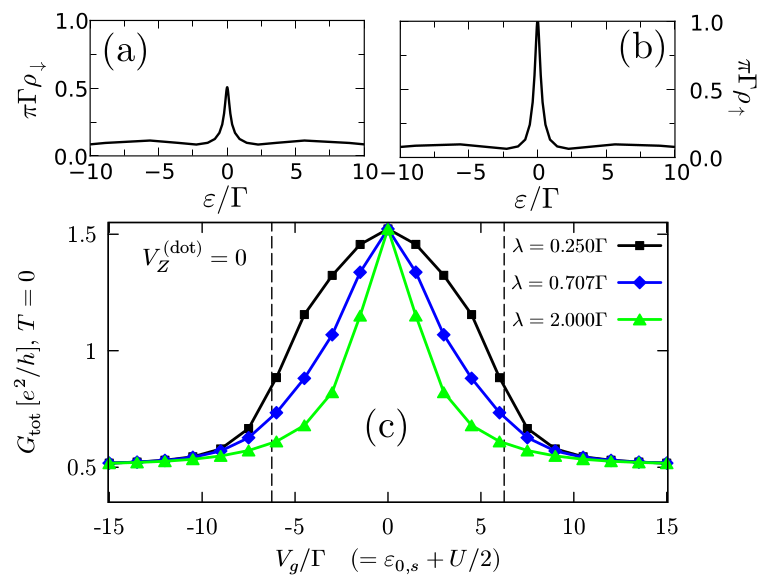
\includegraphics[scale=0.4]{IMAGES/Kondo-MajoranaCond.png}
    \caption{\label{Fig-Kondo-Majorana conductance}(a) QD spin-down
    density of states. Because this channel couples to the Majorana mode,
    it displays the characteristic zero-bias signature of amplitude
    $\frac{e^{2}}{2h}$. (b) QD spin-up density of states,
    displaying the zero-bias peak of the Kondo effect, with
    unit amplitude. (c) Zero-bias conductance of the QD coupled
    to the Majorana mode, as a function of the QD energy level ($\lambda$
    parameterizes the strength of the Majorana-QD tunnel coupling).
    The presence of the spin-up Kondo resonance enhances the
    QD conductance in particle-hole symmetry ($V_{g}=0$),
    but quickly disappears as the QD level is detuned from this point.
    The spin-down Majorana signature, on the other hand, is
    robust {[}7{]}, leaving a residual conductance of $\frac{e^{2}}{2h}$.
    \protect\Source{\citep{ruiz-tijerina_interaction_2015}}.}
\end{figure}

This study revealed that transport measurements
through the quantum dot will show contributions to the enhanced conductance
coming from the Kondo effect and the Majorana mode: The Majorana mode
at the end of the wire will leak into one of the quantum dot spin channels,
giving rise to a zero-mode in the density of states
(\ref{Fig-Kondo-Majorana conductance}a)) contributing a conductance
of $\frac{e^{2}}{2h}$(\ref{Fig-Kondo-Majorana conductance}c)). The
zero\textendash bias peak from the Kondo effect appears in the other
spin channel (\ref{Fig-Kondo-Majorana conductance}b)), contributing
a conductance of $\frac{e^{2}}{h}$. Then, the Kondo effect can be
"turned off" through gate voltages
and magnetic fields, leaving only the Majorana contribution. Clear
evidence of the destruction of the Kondo peak will appear in the conductance,allowing for a distinction between Majorana and Kondo signatures.

 Another insight of this method is the the possibility of manipulating  Majorana fermions  in multidot systems, which recently has turned on new lights into the design of braiding protocols \cite{malciu_braiding_2018}
 of quantum architectures \cite{plugge_majorana_2017,karzig_scalable_2017,barkeshli_physical_2015}.

  The simplest case where Majorana manipulation is possible is in a double quantum dot (DQD). Tunneling Majorana modes in these basic structures have inspired theoretical studies \cite{silva_andreev_2016,ivanov_coherent_2017}
 and experimental setups confirming the observations of Andreev molecules \cite{su_andreev_2017}. Even though quantum tunneling of a MZM into a double dot shows several possibilities for manipulation of MZM,  there is still no complete analysis of the transitions of the Majorana signatures between the QDs in this model.

   In this thesis we fill this gap by performing a transport study of a DQD coupled to a MZM and a metallic lead. The simplicity of this model allows us to explore analytically different geometries of QD's from linear couplings to T-junctions . We considered both non-interacting and interacting regimes, observing major agreement between both approaches about the location of the Majorana signature. While the non-interacting regime is suitable to obtain exact expressions for the Green function, the interacting case  shows how the Majorana signature co-exists with strongly correlated phenomena such as the Kondo effect  and RKKY interactions.   \cite{ruderman_indirect_1954,kasuya_theory_1956,yosida_magnetic_1957} 
  by shifting the QD gate voltages and tunnel couplings which brings possible applications in  braiding procedures. The simplest system where Majorana manipulation is possible is  a  Double Quantum Dot (DQD) coupled to a majorana chain. By tuning the QD gate voltages and the majorana coupling we will be able to probe the mobility of the majorana modes through the dots.
 
% In addition, when both dots are coupled to the lead the Double Quantum Dot exhibits an anti-ferromagnetic interaction known as  Ruderman-Kittel-Kasuya-Yosida (RKKY) \cite{ruderman_indirect_1954,kasuya_theory_1956,yosida_magnetic_1957}. On the other hand, when only one dot is coupled  and the second Dot is indirectly attached through the first dot,  the Kondo effect is annihilated due to the destructive interference  generated by extra dot \cite{dias_da_silva_transmission_2008}. Both cases reveal interesting results for majorana manipulation and hybrid Kondo-Majorana systems.


\section{Overview}

This thesis is integrated by $4$-major chapters:

\begin{itemize}
\item In  \ref{chap:Preliminaries}, we will take a review to the basis of quantum transport in single electron transistors, the Anderson model and the emergence of the Kondo effect in quantum dots. 

 \item In \ref{chap: Methods} we provide a description of the methods that we will use to study the Double Quantum Dot-Majorana system. To study non-interacting systems we will use the Zubarev's ballistic transport\cite{zubarev_double-time_1960} which is optimized through the Graph-Gauss-Jordan elimination algorithm define in \ref{sec:GraphMethod}. For non-interacting systems we use Wilson's Numerical Renormalization Group (NRG) technique \citep{wilson_renormalization_1975}. We will probe our methods in a double quantum dot attached to a magnetic field. Hence, background information about double quantum dots systems will be presented in this chapter. 

\item In \ref{chap:Majorana} we will make a recount of the main topics regarding the pursuit of Majorana fermions in condensed matter systems. This will allow us to motivate the study of Majorana-Kondo coupling in double quantum dots.  We will discuss initial toy models, applications on quantum computing, experimental advances and the innovative idea of coupling Majorana wires with quantum dots. In the last section, we will probe our methods in the QD-Majorana system, and confirm its agreement with previous papers.

 % \item Majorana fermions. The discussion will start with the Kitaev chain addressing its main characteristics such as topological characterization and non-abelian statistics . Then we take a look to the real implementations of majorana chains were we will discuss the most recent experimental accomplishments  in the area.  At the end, we face the the problem of a hybrid Quantum Dot-Majorana system using the methods described in \ref{chap: Methods}.

\item The  \ref{chap:Results}  contains our major contributions to  this area. Using the methods from \ref{chap: Methods} and the previous acquired experience with the double quantum dot and the QD-Majorana model , we study in a  double quantum dot attached to a Majorana zero mode and a metallic lead. We will characterize in this simple model the transitions of the Majorana signature for distinct configurations of the dots. The final results are now part of a paper that we hope to submit for publication in the following months. 
\end{itemize}
 







